\documentclass[aspectratio=169]{beamer}

\usepackage[T1]{fontenc}
\usepackage[scaled]{helvet}
\usepackage{amsmath}
\usepackage{array}
\usepackage{booktabs}
\usepackage[numbers]{natbib}
\usepackage{graphicx}
\usepackage{tikz}
\usetikzlibrary{arrows.meta,calc,positioning}

% -----------------------------------------------------------------------------
% Course template: preserve the supplied theme, logo, progress bar, and 16:9
% format. Only the presentation content is replaced.
% -----------------------------------------------------------------------------
\usetheme[footline,progressbar=fraction]{ChPresentation}
\setbeamertemplate{navigation symbols}{}
\graphicspath{{assets/}{logos/}}

\definecolor{BrainBlue}{HTML}{2466A8}
\definecolor{VisionGreen}{HTML}{238B75}
\definecolor{AccentOrange}{HTML}{D96724}
\definecolor{SoftGray}{HTML}{F1F3F6}
\definecolor{MidGray}{HTML}{596273}
\definecolor{DarkInk}{HTML}{19202C}

\setbeamercolor{normal text}{fg=DarkInk,bg=white}
\setbeamercolor{block title}{fg=white,bg=HAIred}
\setbeamercolor{block body}{fg=DarkInk,bg=HAIred!6}
\setbeamercolor{block title example}{fg=white,bg=VisionGreen}
\setbeamercolor{block body example}{fg=DarkInk,bg=VisionGreen!7}
\setbeamercolor{block title alerted}{fg=white,bg=AccentOrange}
\setbeamercolor{block body alerted}{fg=DarkInk,bg=AccentOrange!8}

% -----------------------------------------------------------------------------
% Fill these three fields after content audit.
% -----------------------------------------------------------------------------
\newcommand{\PresenterName}{YOUR NAME}
\newcommand{\StudentID}{YOUR STUDENT ID}
\newcommand{\TeamMembers}{YOUR TEAM MEMBERS}
\newcommand{\PresentationDate}{Monday, 27 July 2026}

\title[Let Both Sides Adapt]{Let Both Sides Adapt}
\subtitle{Parameter-efficient asymmetric brain--vision alignment\\for EEG image retrieval}
\author{\PresenterName\quad|\quad\StudentID\\[2pt]\TeamMembers\\[2pt]\PresentationDate}
\institute{AIAA3800 --- Human-Centered Artificial Intelligence\\AI Thrust, HKUST (GZ)}
\date{\PresentationDate}
\titlegraphic{
\includegraphics[scale=0.07]{HKUSTGZ.png}}
\framelogo{
\includegraphics[scale=0.047]{HKUSTGZ.png}}

\newcommand{\sourcefooter}[1]{%
  \vfill
  {\color{MidGray}\fontsize{6.7}{8.0}\selectfont Source: #1\par}
}

\newcommand{\metric}[3]{%
  {\color{#1}\bfseries\fontsize{31}{34}\selectfont #2\par}
  \vspace{2pt}
  {\fontsize{13}{16}\selectfont #3\par}
}

\newcommand{\smalllabel}[2]{%
  {\color{#1}\bfseries\fontsize{9.5}{11.5}\selectfont\MakeUppercase{#2}\par}
}

\begin{document}
\backgroundcanvas{}

% =============================================================================
% MAIN TALK
% =============================================================================

\section{Problem}

\begin{frame}{Can 17 EEG channels recover one image from 200?}
% [Sources]
% - Gifford et al. (2022), THINGS-EEG2.
% - README.md, verified standard independent retrieval protocol.
% Speaker note: Define the task before giving the method. This is exact-image
% retrieval from a closed gallery, not class recognition or open-world decoding.
  \vspace{3pt}
  \begin{columns}[T,onlytextwidth]
    \column{0.39\textwidth}
      \smalllabel{BrainBlue}{The task}
      \vspace{5pt}
      {\fontsize{14.5}{17.5}\selectfont
        A person views an image. We ask whether their non-invasive EEG can
        retrieve that \textbf{exact image} from a held-out gallery.
      \par}

      \vspace{6pt}
      {\color{MidGray}\fontsize{10.5}{12.5}\selectfont
        17 posterior channels\\
        250 time samples\\
        repeated-trial averaging
      \par}

    \column{0.57\textwidth}
      \centering
      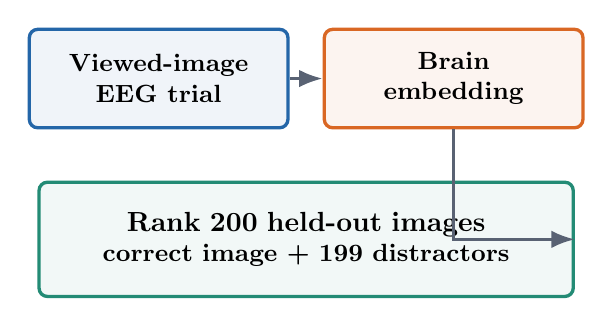
\begin{tikzpicture}[
        node distance=0.42cm,
        box/.style={rounded corners=3pt,draw,very thick,align=center,
          minimum height=1.25cm,text width=3.05cm,font=\small\bfseries},
        arrow/.style={-{Latex[length=3mm]},very thick,color=MidGray}
      ]
        \node[box,draw=BrainBlue,fill=BrainBlue!7] (eeg)
          {Viewed-image\\EEG trial};
        \node[box,draw=AccentOrange,fill=AccentOrange!7,right=of eeg] (embed)
          {Brain\\embedding};
        \draw[arrow] (eeg) -- (embed);
        \node[draw=VisionGreen,fill=VisionGreen!6,rounded corners=3pt,
          very thick,align=center,text width=6.55cm,minimum height=1.45cm,
          below=0.65cm of $(eeg.south)!0.5!(embed.south)$] (gallery)
          {\bfseries Rank 200 held-out images\\[-1pt]
           \fontsize{9.5}{11}\selectfont correct image + 199 distractors};
        \draw[arrow] (embed.south) |- (gallery.east);
      \end{tikzpicture}

      \vspace{5pt}
      \begin{columns}[T,onlytextwidth]
        \column{0.46\textwidth}
          \centering
          {\color{MidGray}\fontsize{10}{12}\selectfont Random Top-1\par}
          {\color{AccentOrange}\bfseries\fontsize{22}{25}\selectfont 0.5\%\par}
        \column{0.46\textwidth}
          \centering
          {\color{MidGray}\fontsize{10}{12}\selectfont Our five-seed Top-1\par}
          {\color{BrainBlue}\bfseries\fontsize{22}{25}\selectfont 86.66\%\par}
      \end{columns}
  \end{columns}
  \sourcefooter{THINGS-EEG2; project fixed-checkpoint 200-way exact-image retrieval protocol.}
\end{frame}

\begin{frame}{A rigid visual space makes EEG carry the whole mismatch}
% [Sources]
% - Project design rationale in docs/brain_rw_progress.md.
% - train_clip_lora.py implementation.
% Speaker note: Set up the design tension. Frozen vision is stable but rigid;
% full fine-tuning moves too much for a small, noisy human-signal dataset.
  \vspace{4pt}
  \begin{columns}[T,onlytextwidth]
    \column{0.46\textwidth}
      \begin{block}{Freeze the visual encoder}
        \vspace{2pt}
        {\fontsize{13.5}{17}\selectfont
          Preserves CLIP's pretrained semantics, but forces the EEG encoder
          to absorb the entire cross-modal gap.
        \par}
      \end{block}

    \column{0.46\textwidth}
      \begin{alertblock}{Fully fine-tune the visual encoder}
        \vspace{2pt}
        {\fontsize{13.5}{17}\selectfont
          Lets vision move freely, but small EEG datasets make overfitting
          and loss of the pretrained visual prior more likely.
        \par}
      \end{alertblock}
  \end{columns}

  \vspace{13pt}
  \begin{center}
    {\color{MidGray}\fontsize{13}{16}\selectfont
      The two modalities should meet in the middle ---
    \par}
    \vspace{3pt}
    {\color{HAIred}\bfseries\fontsize{21}{25}\selectfont
      while vision moves less.
    \par}
  \end{center}
  \sourcefooter{Project rationale and implemented optimizer structure.}
\end{frame}

\section{Method}

\begin{frame}{EEG learns fast; vision adapts slowly}
% [Sources]
% - train_clip_lora.py: LoRA target modules and optimizer parameter groups.
% - main/models_brain.py and main/models_clip.py.
% - README.md: verified locked configuration.
% Speaker note: This is the method slide. The brain model is fully trained;
% only the vision branch uses LoRA. We combine known tools into an asymmetric
% adaptation rule designed for small, noisy EEG data.
  \smalllabel{HAIred}{Our method: asymmetric co-adaptation}
  \vspace{7pt}
  \centering
  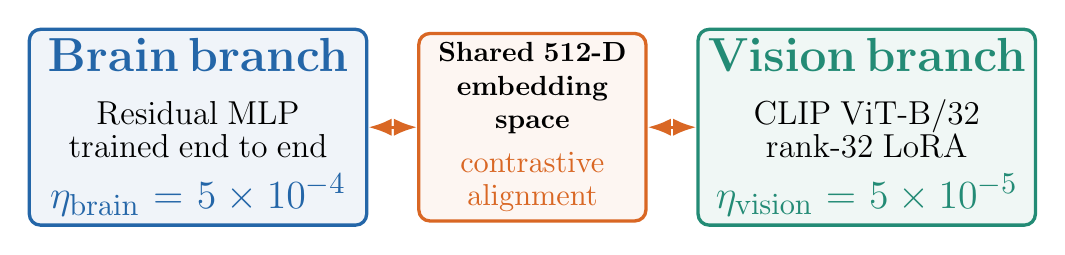
\begin{tikzpicture}[
    branch/.style={rounded corners=4pt,very thick,align=center,
      minimum height=2.45cm,text width=4.05cm},
    shared/.style={rounded corners=4pt,very thick,align=center,
      minimum height=1.65cm,text width=2.65cm},
    flow/.style={<->,>=Latex,very thick,color=AccentOrange}
  ]
    \node[branch,draw=BrainBlue,fill=BrainBlue!7] (brain) {
      {\color{BrainBlue}\bfseries\fontsize{17}{20}\selectfont Brain branch}\\[5pt]
      {\fontsize{11.5}{14}\selectfont Residual MLP\\trained end to end}\\[5pt]
      {\color{BrainBlue}\bfseries\fontsize{15}{18}\selectfont
        $\eta_{\mathrm{brain}}=5\times10^{-4}$}
    };
    \node[shared,draw=AccentOrange,fill=AccentOrange!6,right=0.62cm of brain] (space) {
      {\bfseries Shared 512-D\\embedding space}\\[4pt]
      {\color{AccentOrange}\fontsize{10.5}{13}\selectfont contrastive alignment}
    };
    \node[branch,draw=VisionGreen,fill=VisionGreen!7,right=0.62cm of space] (vision) {
      {\color{VisionGreen}\bfseries\fontsize{17}{20}\selectfont Vision branch}\\[5pt]
      {\fontsize{11.5}{14}\selectfont CLIP ViT-B/32\\rank-32 LoRA}\\[5pt]
      {\color{VisionGreen}\bfseries\fontsize{15}{18}\selectfont
        $\eta_{\mathrm{vision}}=5\times10^{-5}$}
    };
    \draw[flow] (brain) -- (space);
    \draw[flow] (space) -- (vision);
  \end{tikzpicture}

  \vspace{9pt}
  {\color{HAIred}\bfseries\fontsize{18}{22}\selectfont
    Brain updates are 10$\times$ faster than visual updates.
  \par}
  \vspace{2pt}
  {\color{MidGray}\fontsize{10.5}{13}\selectfont
    Vision adapts through all-linear LoRA; the pretrained CLIP weights remain frozen.
  \par}
  \sourcefooter{Brain residual MLP; CLIP ViT-B/32; LoRA rank/alpha 32; branch learning rates 5e-4 and 5e-5.}
\end{frame}

\begin{frame}{The training objective matches independent retrieval}
% [Sources]
% - main/models_clip.py: L2 normalization, similarity matrix, and one-direction
%   brain-to-image contrastive loss.
% - train_clip_lora.py: independent 200-image gallery ranking.
% Speaker note: Do not call the loss symmetric. The implementation optimizes
% contrastive_loss(logits_per_brain). Standard evaluation independently ranks
% every query; Hungarian is excluded.
  \vspace{2pt}
  \begin{columns}[T,onlytextwidth]
    \column{0.47\textwidth}
      \smalllabel{BrainBlue}{Training}
      \vspace{5pt}
      \[
        z_i^b=\frac{E_b(b_i)}{\lVert E_b(b_i)\rVert_2},
        \qquad
        z_j^v=\frac{E_v(x_j)}{\lVert E_v(x_j)\rVert_2}
      \]
      \[
        S_{ij}=\exp(\alpha)\,(z_i^b)^\top z_j^v
      \]
      {\fontsize{12.2}{15.5}\selectfont
        Brain-to-image contrastive loss pushes each paired image above
        the other images in the batch.
      \par}

    \column{0.47\textwidth}
      \smalllabel{VisionGreen}{Evaluation}
      \vspace{7pt}
      {\color{VisionGreen}\bfseries\fontsize{16}{20}\selectfont
        One EEG query
      \par}
      \vspace{5pt}
      {\color{AccentOrange}\bfseries\fontsize{18}{22}\selectfont
        $\downarrow$ 200 cosine scores $\downarrow$
      \par}
      \vspace{5pt}
      {\color{DarkInk}\bfseries\fontsize{16}{20}\selectfont
        Independent Top-1 / Top-5 ranking
      \par}
      \vspace{8pt}
      {\color{MidGray}\fontsize{11}{14}\selectfont
        No one-to-one assignment and no Hungarian decoding in the standard result.
      \par}
  \end{columns}

  \sourcefooter{Repository implementation and audited fixed-checkpoint evaluation protocol.}
\end{frame}

\section{Evidence}

\begin{frame}{The complete system retrieves the viewed image reliably}
% [Sources]
% - README.md, five-seed ten-subject standard independent retrieval.
% Speaker note: The uncertainty is the sample SD across five seed-level
% ten-subject macro scores. The 10,000 query evaluations repeat the same
% held-out stimuli across seeds and are not 10,000 independent examples.
  \smalllabel{BrainBlue}{Main system: 10 subjects $\times$ 5 seeds}
  \vspace{12pt}
  \begin{columns}[T,onlytextwidth]
    \column{0.47\textwidth}
      \centering
      \metric{BrainBlue}{86.66\%}{Top-1 accuracy\\
        {\color{MidGray}$\pm$ 0.69 percentage points}}

    \column{0.47\textwidth}
      \centering
      \metric{VisionGreen}{98.38\%}{Top-5 accuracy\\
        {\color{MidGray}$\pm$ 0.14 percentage points}}
  \end{columns}

  \vspace{14pt}
  {\color{HAIred}\rule{\textwidth}{1.5pt}}
  \vspace{6pt}
  \begin{columns}[T,onlytextwidth]
    \column{0.32\textwidth}
      \centering
      {\color{MidGray}\fontsize{10}{12}\selectfont 200-way chance\par}
      {\bfseries\fontsize{15}{18}\selectfont 0.5\% / 2.5\%\par}
    \column{0.32\textwidth}
      \centering
      {\color{MidGray}\fontsize{10}{12}\selectfont Top-1 seed range\par}
      {\bfseries\fontsize{15}{18}\selectfont 85.60--87.35\%\par}
    \column{0.32\textwidth}
      \centering
      {\color{MidGray}\fontsize{10}{12}\selectfont Checkpoint rule\par}
      {\bfseries\fontsize{15}{18}\selectfont fixed epoch 25\par}
  \end{columns}
  \sourcefooter{Five seed-level subject macros; 200 held-out queries per subject--seed model.}
\end{frame}

\begin{frame}{Fifty independent runs converge to the same operating point}
% [Sources]
% - presentation_draft/figures/training_dynamics_50_runs.pdf.
% - presentation_draft/figures/README.md for metric provenance.
% Speaker note: These trajectories are post-hoc diagnostics on the formal test
% split. They show stability, but they were never used to choose a checkpoint.
  \vspace{-3pt}
  \centering
  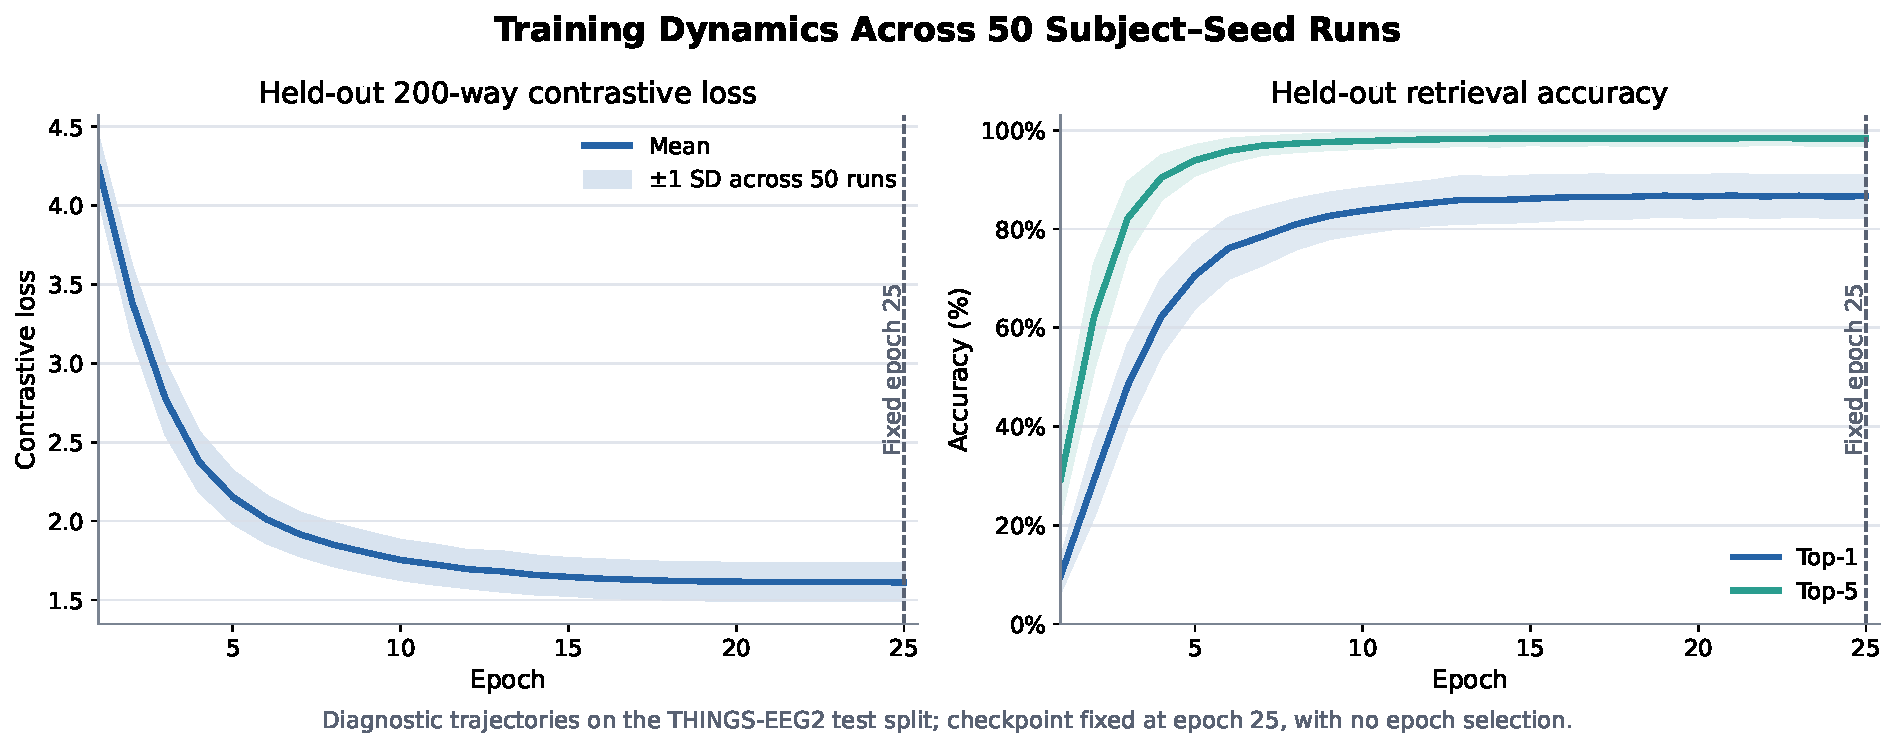
\includegraphics[width=0.99\linewidth,height=0.70\textheight,keepaspectratio]
    {training_dynamics_50_runs.pdf}

  \vspace{1pt}
  {\color{HAIred}\bfseries\fontsize{10.5}{13}\selectfont
    Every reported model uses epoch 25; the curves are diagnostics, not model selection.
  \par}
  \sourcefooter{50 subject--seed trajectories: seeds 42--46, subjects 01--10.}
\end{frame}

\begin{frame}{Matched control isolates a +6.51-point gain}
% [Sources]
% - experiments/samga_lora/README.md, confirmatory paired study.
% - docs/protocols/SAMGA_LORA_EXPERIMENT_PLAN_ZH.md.
% Speaker note: This is a separate SAMGA-style system. The value of the
% experiment is isolation of the intervention, not direct comparison with the
% 86.66% main system.
  \smalllabel{AccentOrange}{Controlled attribution --- separate SAMGA-style system}
  \vspace{3pt}

  \begin{center}
    \renewcommand{\arraystretch}{1.28}
    \begin{tabular}{>{\raggedright\arraybackslash}p{6.0cm}cc}
      \toprule
      \textbf{Matched visual arm} & \textbf{Top-1} & \textbf{Top-5}\\
      \midrule
      Frozen CLIP & 76.17\% & 95.79\%\\
      + visual LoRA/TTUR & \textbf{\color{VisionGreen}82.68\%}
                         & \textbf{\color{VisionGreen}97.67\%}\\
      \bottomrule
    \end{tabular}
  \end{center}

  \vspace{2pt}
  \begin{center}
    {\color{AccentOrange}\bfseries\fontsize{27}{31}\selectfont +6.51 points\par}
    {\color{MidGray}\fontsize{11.5}{14}\selectfont
      95\% CI: [+5.22, +7.69]
    \par}
  \end{center}

  \vspace{1pt}
  \begin{columns}[T,onlytextwidth]
    \column{0.48\textwidth}
      \centering{\bfseries\fontsize{13}{16}\selectfont 48 / 50 paired cells improved\par}
    \column{0.48\textwidth}
      \centering{\bfseries\fontsize{13}{16}\selectfont All 10 subjects improved on average\par}
  \end{columns}
  \sourcefooter{Matched 10-subject $\times$ 5-seed study; two-way subject/seed cluster bootstrap, 10,000 resamples.}
\end{frame}

\section{Human-Centered Boundaries}

\begin{frame}{Retrieval accuracy is not mind reading}
% [Sources]
% - README.md, scope, reproducibility policy, and responsible-use boundaries.
% Speaker note: This slide is central to the HAI framing. Accuracy and claim
% discipline are both parts of system quality when working with human data.
  % textpos occasionally drops the theme's inherited frame logo on this block
  % layout, so place the same authentic template asset in the identical slot.
  \begin{textblock*}{100mm}(0.86\linewidth,-4.2ex)
    
\includegraphics[scale=0.043]{HKUSTGZ.png}
  \end{textblock*}
  \vspace{3pt}
  \begin{columns}[T,onlytextwidth]
    \column{0.46\textwidth}
      \begin{exampleblock}{The evidence supports}
        \begin{itemize}
          \item Within-subject retrieval
          \item Trial-averaged EEG
          \item A closed 200-image gallery
          \item Stable five-seed performance
        \end{itemize}
      \end{exampleblock}

    \column{0.46\textwidth}
      \begin{alertblock}{It does not support}
        \begin{itemize}
          \item Cross-subject generalization
          \item Single-trial ``mind reading''
          \item Open-world reconstruction
          \item Clinical or diagnostic use
        \end{itemize}
      \end{alertblock}
  \end{columns}

  \vspace{10pt}
  \begin{center}
    {\color{HAIred}\bfseries\fontsize{14.5}{18}\selectfont
      Consent, privacy, fixed evaluation rules, and restrained claims\\
      are part of the model's human-centered quality.
    \par}
  \end{center}
  \sourcefooter{Project limitations, evaluation policy, and responsible-use statement.}
\end{frame}

\begin{frame}{Let the two modalities meet halfway}
% [Sources]
% - Synthesis of the implemented method and verified result lines.
% Speaker note: Resolve the opening tension, then end on the next scientific
% question rather than on another number.
  \vspace{3pt}
  \begin{center}
    {\color{MidGray}\fontsize{13}{16}\selectfont
      Do not force EEG into a rigid visual space.
    \par}
    \vspace{4pt}
    {\color{HAIred}\bfseries\fontsize{21}{25}\selectfont
      Let EEG learn fast, while vision adapts slowly.
    \par}
  \end{center}

  \vspace{12pt}
  \begin{columns}[t,onlytextwidth]
    \column{0.30\textwidth}
      \begin{block}{\centering Asymmetric}
        \centering
        {\fontsize{11.5}{14}\selectfont
          Brain updates 10$\times$ faster than vision.
        \par}
      \end{block}

    \column{0.30\textwidth}
      \begin{exampleblock}{\centering Efficient}
        \centering
        {\fontsize{11.5}{14}\selectfont
          Rank-32 LoRA preserves the CLIP prior.
        \par}
      \end{exampleblock}

    \column{0.30\textwidth}
      \begin{alertblock}{\centering Supported}
        \centering
        {\fontsize{11.5}{14}\selectfont
          Strong main result and matched-control gain.
        \par}
      \end{alertblock}
  \end{columns}

  \vspace{7pt}
  \begin{center}
    {\color{MidGray}\fontsize{11}{14}\selectfont
      Next: test whether the principle survives cross-subject and single-trial settings.
    \par}
  \end{center}
\end{frame}

\begin{frame}[plain,noframenumbering]
  \vspace{68pt}
  \centering
  {\color{HAIred}\bfseries\fontsize{27}{31}\selectfont Thank you!\par}
  \vspace{9pt}
  {\fontsize{17}{21}\selectfont Questions?\par}
\end{frame}

% =============================================================================
% BACKUP
% =============================================================================

\appendix

\begin{frame}{Backup: Full training and retrieval pipeline}
% [Sources]
% - Project-authored asset: asserts/Architecture.png.
  \centering
  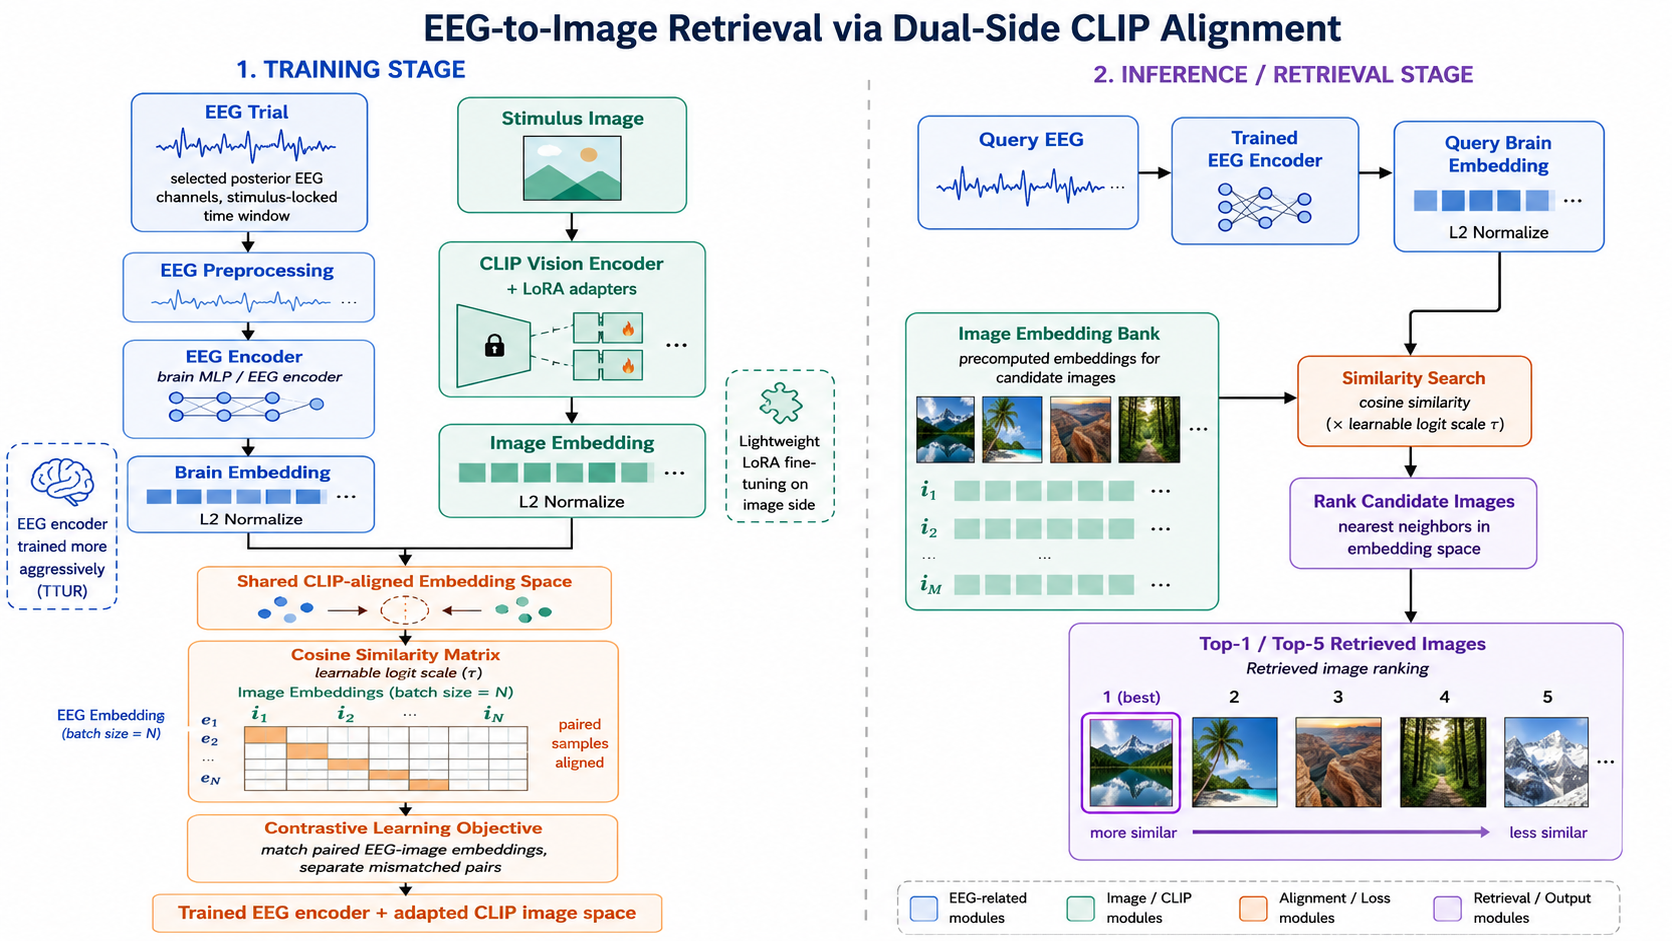
\includegraphics[width=0.99\linewidth,height=0.80\textheight,keepaspectratio]
    {Architecture.png}
  \sourcefooter{Project-authored architecture visual.}
\end{frame}

\begin{frame}{Backup: Verified final LoRA configuration}
% [Sources]
% - presentation_draft/figures/lora_final_configuration.pdf.
  \centering
  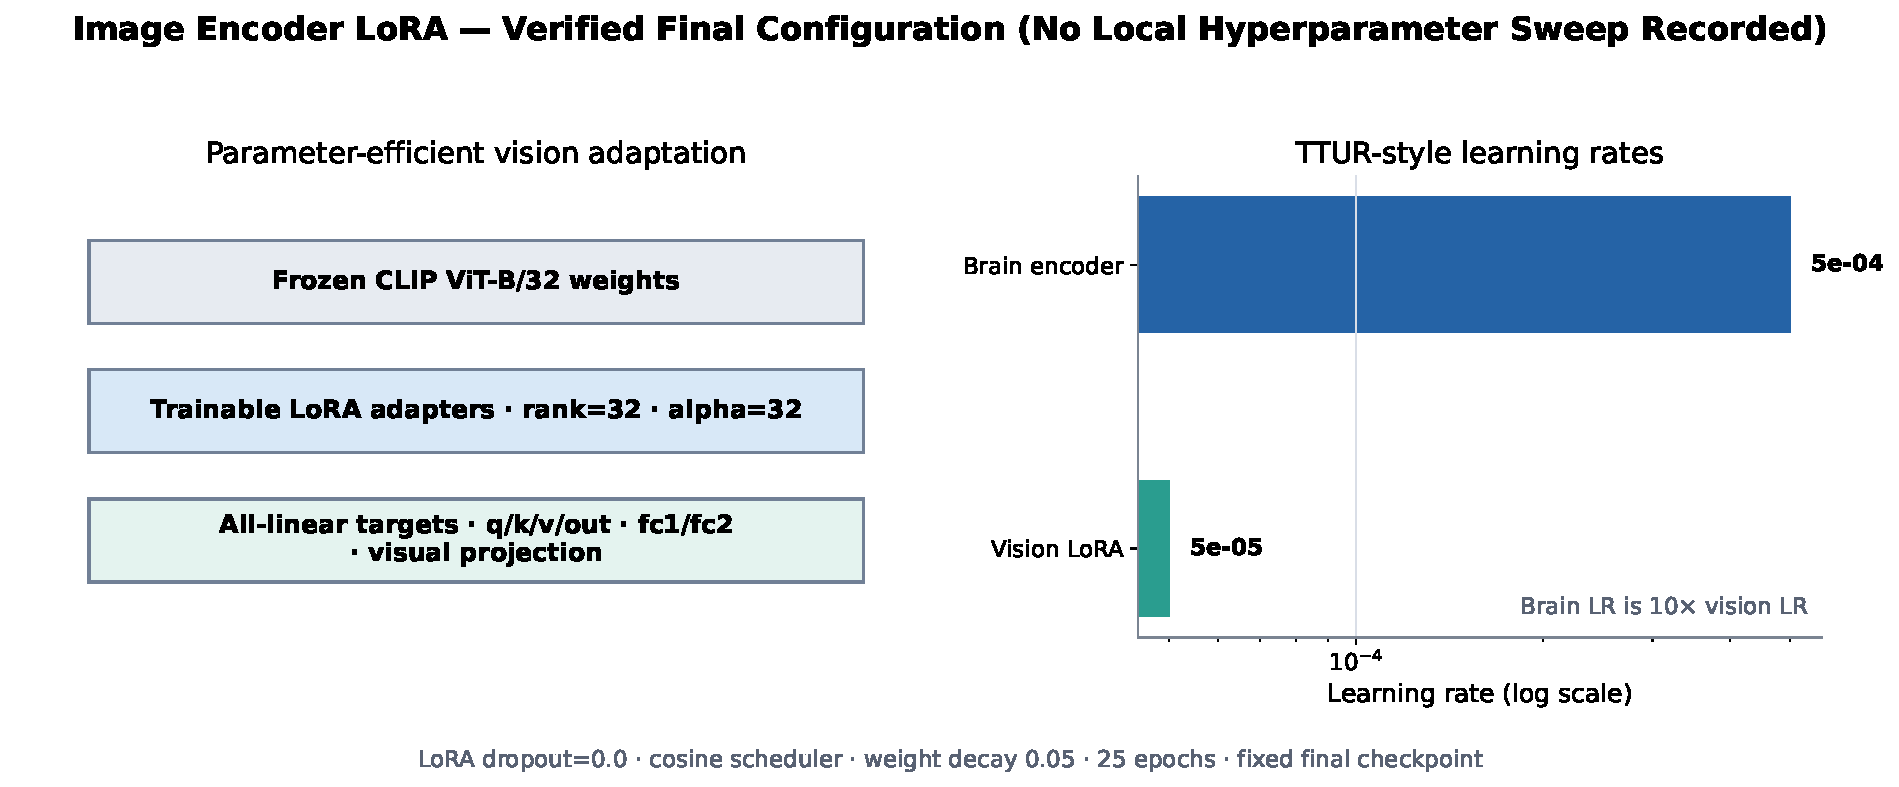
\includegraphics[width=0.99\linewidth,height=0.73\textheight,keepaspectratio]
    {lora_final_configuration.pdf}
  \vspace{2pt}
  {\color{HAIred}\bfseries\fontsize{9.5}{11.5}\selectfont
    This documents the final configuration; no local sweep supports an optimality claim.
  \par}
  \sourcefooter{Verified project configuration; rank/alpha 32, dropout 0, cosine schedule, weight decay 0.05, 25 epochs.}
\end{frame}

\begin{frame}{Backup: Literature comparison is contextual}
% [Sources]
% - presentation_draft/figures/literature_baseline_comparison_no_samga.pdf.
% - README.md literature table and protocol caveats.
  \centering
  {\color{HAIred}\bfseries\fontsize{9.7}{11.8}\selectfont
    Protocols differ; SAMGA is intentionally omitted from this plot; no unqualified SOTA claim.
  \par}
  \vspace{2pt}
  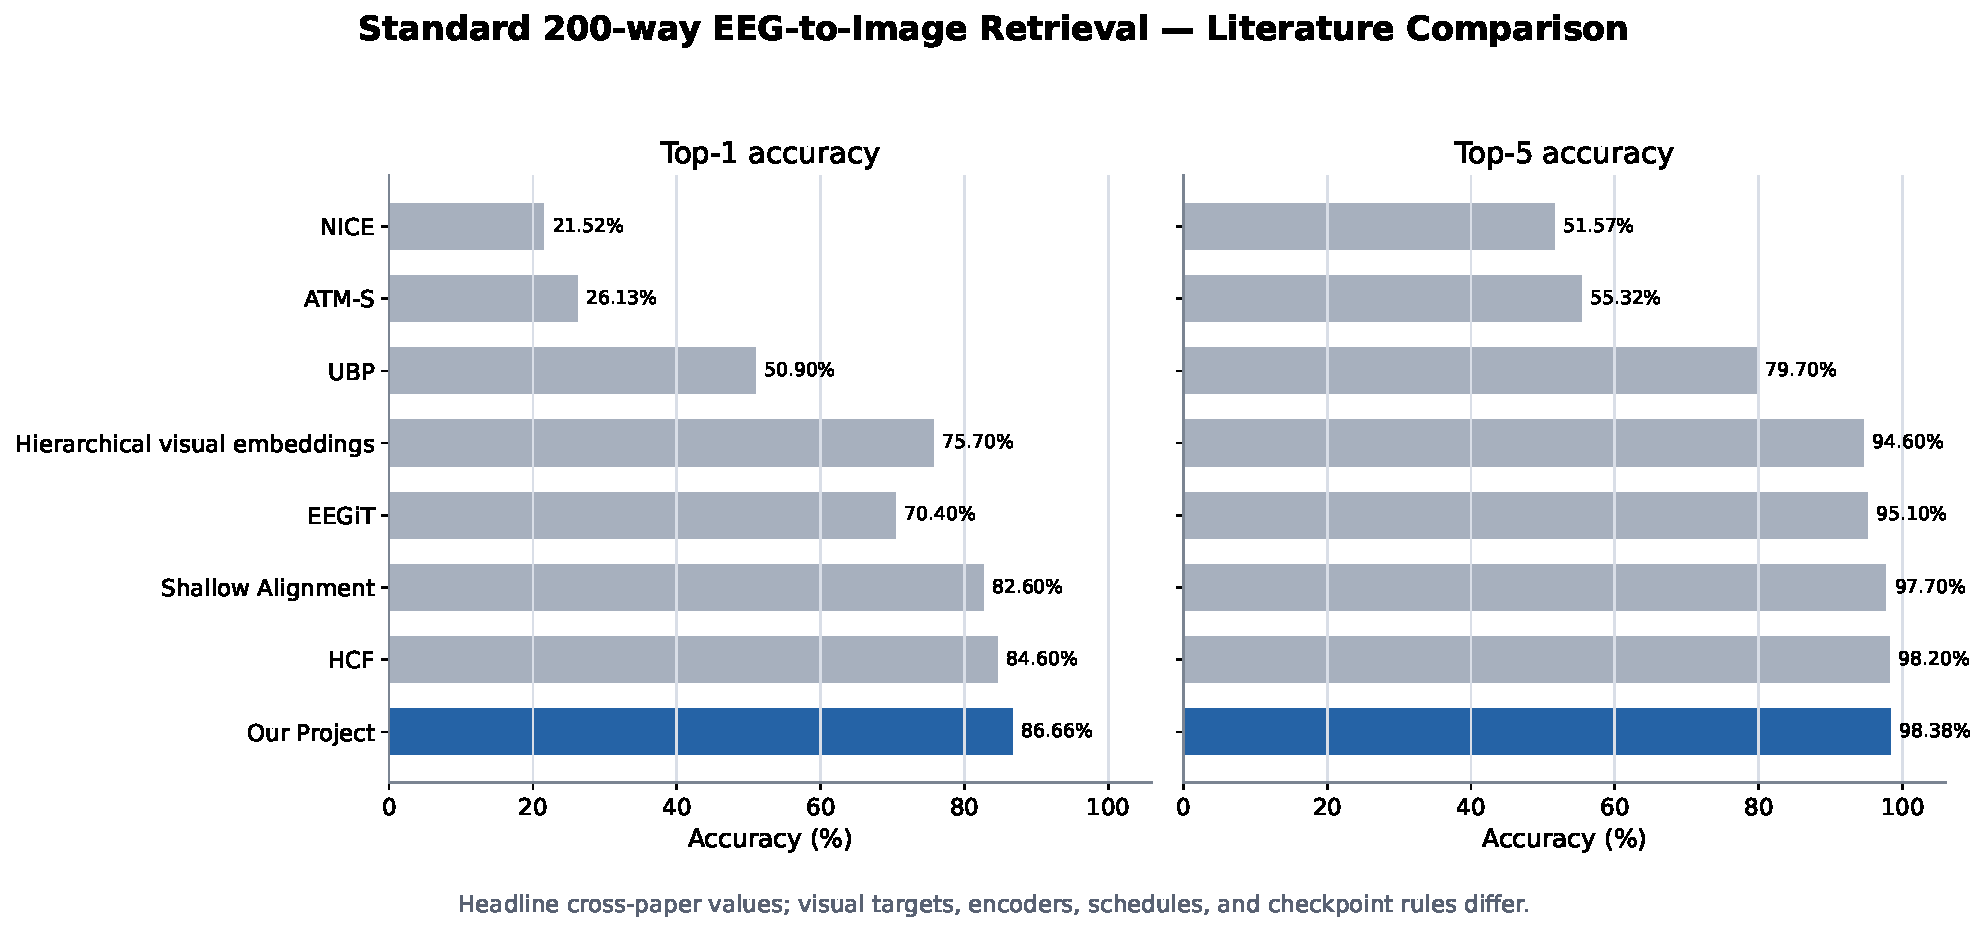
\includegraphics[width=0.99\linewidth,height=0.70\textheight,keepaspectratio]
    {literature_baseline_comparison_no_samga.pdf}
  \sourcefooter{Headline cross-paper values; visual targets, encoders, schedules, and checkpoint rules differ.}
\end{frame}

\begin{frame}{Backup: Global assignment is a transductive diagnostic}
% [Sources]
% - presentation_draft/figures/local_baseline_comparison_sub08_seed42.pdf.
% - README.md Hungarian ablation.
  \centering
  {\color{HAIred}\bfseries\fontsize{9.7}{11.8}\selectfont
    Subject-08, seed 42 only; global methods inspect the complete similarity matrix.
  \par}
  \vspace{2pt}
  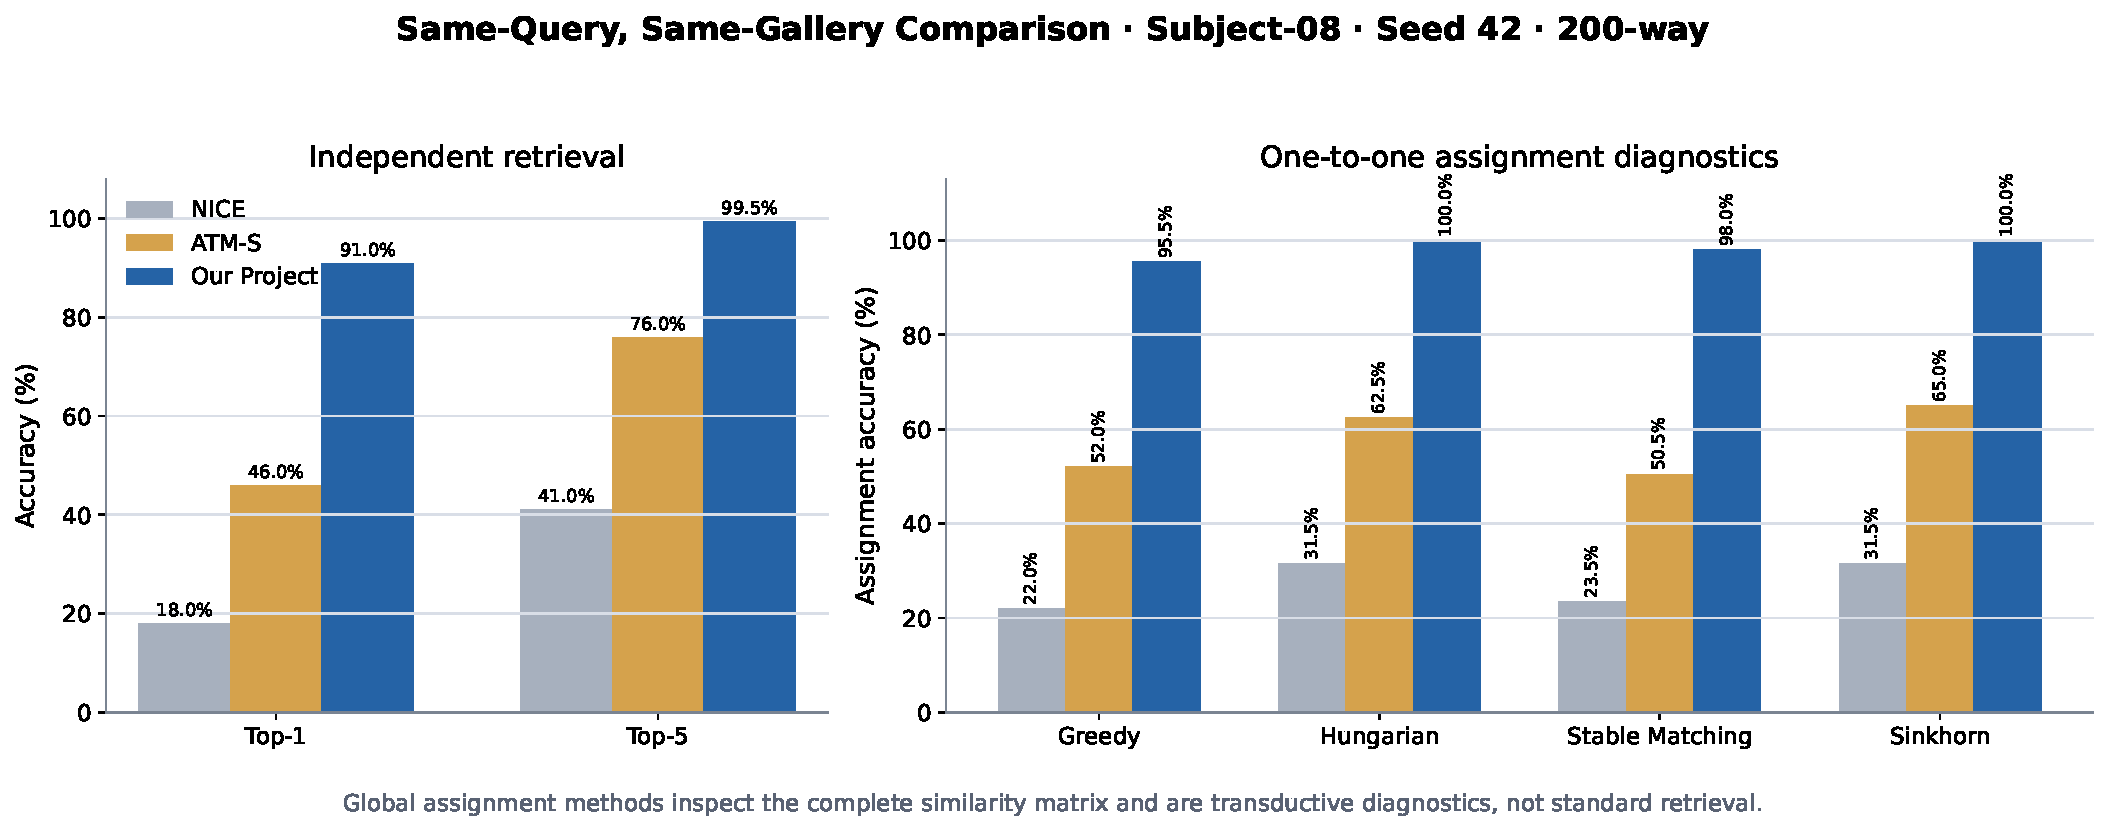
\includegraphics[width=0.99\linewidth,height=0.70\textheight,keepaspectratio]
    {local_baseline_comparison_sub08_seed42.pdf}
  \sourcefooter{Same-query, same-gallery local comparison; Hungarian is excluded from every standard aggregate.}
\end{frame}

\begin{frame}{Backup: Five result tracks remain separate}
% [Sources]
% - README.md and docs/brain_rw_progress.md.
  \vspace{2pt}
  \begin{center}
    {\fontsize{10.5}{12.7}\selectfont
    \renewcommand{\arraystretch}{1.08}
    \begin{tabular}{>{\bfseries\raggedright\arraybackslash}p{3.35cm}
                    >{\raggedright\arraybackslash}p{8.55cm}}
      \toprule
      Track & Correct interpretation\\
      \midrule
      Main system &
      Fixed epoch-25 independent retrieval: 86.66\% / 98.38\%.\\
      Controlled LoRA &
      Matched Frozen vs.\ LoRA/TTUR test in a SAMGA-style system.\\
      SAMGA reproduction &
      Audited approximation; separate from our main method.\\
      Hungarian &
      One Subject-08/seed-42 transductive diagnostic.\\
      Reconstruction &
      Exploratory extension without a formal headline result.\\
      \bottomrule
    \end{tabular}
    }
  \end{center}
  \sourcefooter{Repository result taxonomy and claim boundaries.}
\end{frame}

\begin{frame}{References}
  \nocite{things,clip,lora,atm,samga}
  \bibliographystyle{abbrvnat}
  {\fontsize{7.5}{9.2}\selectfont\bibliography{ref}}
\end{frame}

\end{document}
